\documentclass{article}

\usepackage{tikz}

\newlength{\step}

\begin{document}
  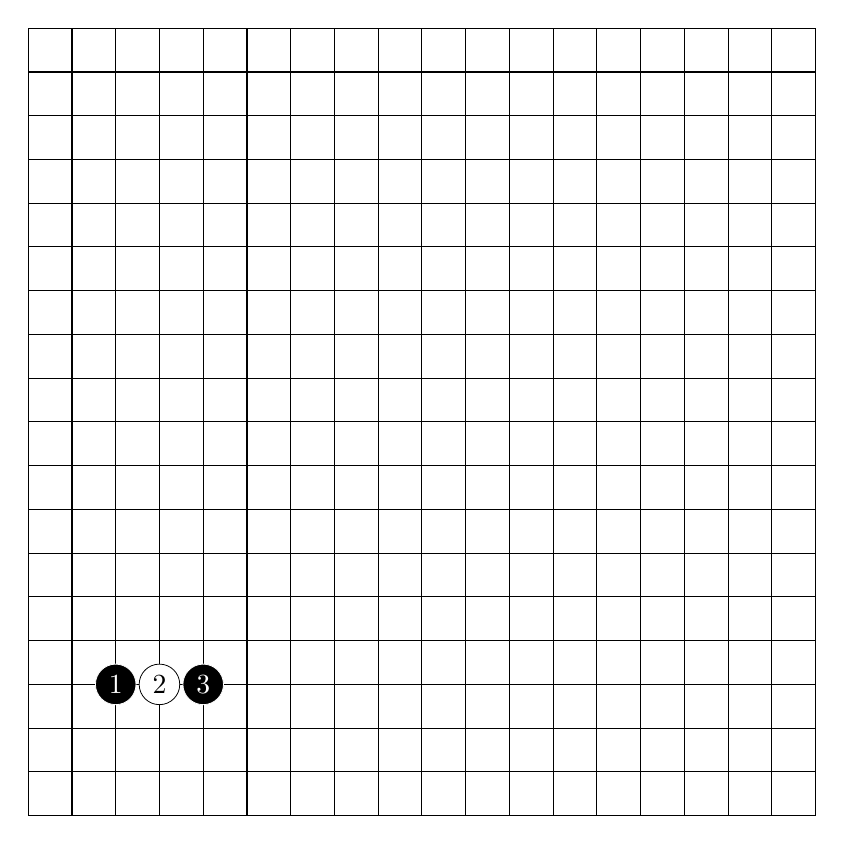
\begin{tikzpicture}
    \setlength{\step}{\dimexpr 10cm / 18 \relax}

    \draw[step=\step] (0, 0) grid (10, 10);

    \draw[draw = white, line width = 0.1mm, fill = black]
      (2 * 10cm / 18, 3 * 10cm / 18) circle [radius = 0.2575cm]
      node[color = white] {1};
    \draw[draw = black, line width = 0.1mm, fill = white]
      (3 * 10cm / 18, 3 * 10cm / 18) circle [radius = 0.2575cm]
      node[color = black] {2};
    \draw[draw = white, line width = 0.1mm, fill = black]
      (4 * 10cm / 18, 3 * 10cm / 18) circle [radius = 0.2575cm]
      node[color = white] {3};
  \end{tikzpicture}
\end{document}